\chapter{Introduction}

Rapid situational awareness is the key to enabling a successful response from first responders during an emergency. Incident command uses all information available to them to make decisions and coordinate the first responders. First responders are often sent into the incident scene to gather information, but the nature of emergencies makes this process dangerous and can risk additional lives. Subterranean environments pose a number of additional hazards and challenges, such as outdated maps, dangerous terrain, and low visibility, making them particularly difficult to send humans into safely. For example, emergency personnel cannot safely explore beyond fires in coal mines, and are thus unable to determine the number of people or quality of terrain that may be behind them. Autonomous systems have the potential to significantly improve the quality and timeliness of the situational awareness gained in challenging subterranean environments, and by doing so can reduce risk to human lives.

% Livestream: https://www.youtube.com/watch?v=rMW-wZTecqE (2:47:00 mark or so for the MSHA presentation)
% NYC fire chief: https://www.youtube.com/watch?v=4I4J67jxODE

\section{The DARPA Subterranean Challenge (SubT)}

The DARPA Subterranean Challenge was issue to spur the development of new technologies to explore these complex underground environments. Teams are challenged to propose new and innovative solutions for the unique perception, mobility, communication, and autonomy problems present in these environments. Teams compete in a series of 3 separate circuit events, each in a different type of subterranean environment, listed in Figure \ref{darpa_environments}. The highest performing teams will be invited to a final event which incorporates elements of each type of environment. In each event, teams are tasked with deploying systems which rapidly provide situational awareness, in the form of map data and locations of predetermined artifacts placed by DARPA.

\begin{figure}	
	\centering
	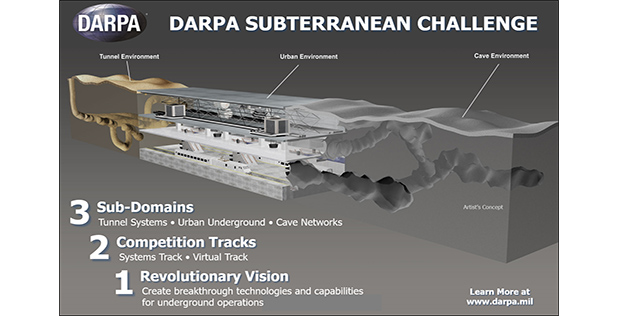
\includegraphics[width=\textwidth]{darpa_environments.jpg}
	\caption[DARPA Subterranean Challenge environments]{The Tunnel Circuit focuses on human made tunnel systems. The Urban Circuit focuses on urban environments such as mass transit and municipal infrastructure. The Cave Circuit focuses on naturally occurring cave systems.}
	\label{darpa_environments}
\end{figure}

During each circuit event, teams have 60 minutes to deploy their systems in the environment. The deployment may consist of as many robots as the teams desire, but must be operated by a single human supervisor at the team's base station. Not all areas of the environment will be traversable for all types of robots, so teams are encouraged to develop systems with a variety of mobility capabilities. Communication with and coordination of each robot in the fleet is an additional challenge as no communication infrastructure is provided by DARPA. Autonomous exploration capability is advised to reduce operator load and eliminate a need for constant connectivity. The perception systems used to drive the autonomy should be able to handle a variety of challenging conditions, such as low visibility and variable lighting. Teams may be permitted multiple runs per event.

Before a team's run, DARPA places a predetermined and disclosed number of artifacts in the environment. The locations of specific points on each of these artifacts, referenced to a DARPA-defined frame, are surveyed and treated as ground truth. The location of each artifact and number of each artifact type is unknown to teams. Scoring for each competition event is based entirely on the number of artifacts which are correctly reported to DARPA within the 60 minute period. Teams must report the artifact's category and must report coordinates which are within 5m Euclidean distance of the ground truth for an artifact report to be considered correct. Teams may submit twice the number of artifact reports as there are artifacts in the environment. Artifact reports may be generated in whichever manner a team deems appropriate, such as randomly, by the human supervisor, or fully autonomously by the deployed system. Ties between multiple teams are broken by a number of factors, including the times artifacts were submitted, and the furthest artifacts detected.

%https://subtchallenge.com/resources/SubT\_Challenge\_Tunnel\_Rules.pdf
%https://subtchallenge.com/resources/SubT\_Tunnel\_Artifacts\_Specification.pdf

\section{Tunnel Circuit Specifics}

This work focuses specifically on artifact detection and localization in the context of the Tunnel Circuit. The Tunnel Circuit event took place between at the National Institute for Occupational Safety and Health Mining (NIOSH) site in Pittsburgh, PA, between August 15 and August 22 2019. DARPA divided the former coal mine into two separate courses, starting at the mine's two separate portals, Safety Research and Experimental. A map of the Safety Research course is shown in Figure \ref{tunnel_circuit_day_2}. Each team was allowed 2 runs in each course. The team's final score is a sum of the highest score from each course.

20 artifacts were deployed by DARPA in each course. The placement and distribution of artifacts varied between each course and each run, as indicated in Table \ref{final_scores}. Five specific categories of artifacts were used at the Tunnel Circuit, shown in Figure \ref{tunnel artifacts} and described below. Each category of artifact is specified to only use the single model of object shown the figure.

\subsubsection{Backpack}

The backpack artifact represents a typical adult-sized bag for carrying items. The backpack may be found on the ground, on a wall, or resting on a work surface, such as a table. The backpack contains a sandbag to help keep it in place during the competition. The front backpack is facing outward or upward depending on the initial placement.

\subsubsection{Cell Phone}

The cell phone artifact represents a radio used for communication, as well as other typical handheld devices. The cell phone is playing an unspecified full-screen video. Audio is playing from the phone at maximum volume. A 2.4 GHz access point is created by each cell artifact with an SSID of the form "PhoneArtifact\#\#", where "\#\#" is a unique two digit number. The cell phone's Bluetooth radio is on and discoverable.

\subsubsection{Drill}

The drill artifact represents a typical handheld tool. The drill has a Philips head driver in its chuck. The artifact may be found on the ground or on work tables. The orientation of the drill is not specified. The drill is not powered during scored runs.

\subsubsection{Fire Extinguisher}

The fire extinguisher artifact represents a typical common handheld fire extinguisher. This artifact also represents areas where other emergency equipment may be located. The fire extinguisher has its hose in the stored configuration. It may be found on the ground, on a work surface, or hanging from a wall. It will not be used during the scored runs.

\subsubsection{Survivor ("Randy")}

The survivor artifact represents a human survivor, such as a trapped worker. A thermal manikin is used, and is wearing a high visibility jacket, work pants, and standard steel toed work boots. The manikin has heating elements in its hands and head to partially emulate a human's thermal signature. The manikin is not actuated and will not be playing auditory clues. The manikin is placed in a static sitting position against walls.

\section{Our Approach}

Our team's overall concept of operations is one of modular autonomy. We aim to develop a set of hardware and software components that can be rapidly reconfigured and adapted to support the needs of any particular environment. Individual modules can be upgraded or replaced as necessary. For mobility, modules such as removable battery packs, wheel assemblies, and drive electronics are used. For communication, custom nodes are developed, multiples of which can be stored on modular node dropper assemblies. For perception, this approach means the development of various sensing payloads with integrated software and computation that can be transferred between robots. These sensing payloads run modular state estimation and artifact detection and localization software which can adapt to the capabilities of each system.

Within each sensing payload, we use a multimodal suite of sensors for artifact detection. Though a single sensor or category of sensors, such as RGB cameras, may be able to detect multiple types of artifacts, it is unlikely to be able to perform well in all conditions. Alternatively, individual sensors may be particularly well suited to detect a specific artifact easily, but may not detect others at all. For example, the survivor and cell phone artifacts emit a thermal signature that may be able to be detected in a thermal camera, leading to the localization of these artifacts even in cases of little to no light. A WiFi radio may be used to detect and localize which is beyond line of sight, but is incapable of detecting any other categories of artifacts. Using a multimodal suite of sensors with intelligent fusion allows us to exploit the strengths of each individual sensor and create a more accurate and robust overall system.

The human supervisor is also considered a module in our system. Though each robot in the system is capable of autonomous operation, the human supervisor is able to combine course and map information reported from multiple robots and direct the exploration patterns of the fleet. Each robot also returns artifact information to the base station, which the human supervisor aggregates and verifies. Artifacts reports which have been approved by the human supervisor are sent to DARPA at the human supervisor's discretion, and are modified and resubmitted as more information becomes available if necessary.

\begin{figure}
	\centering
	\begin{subfigure}{0.32\textwidth}
		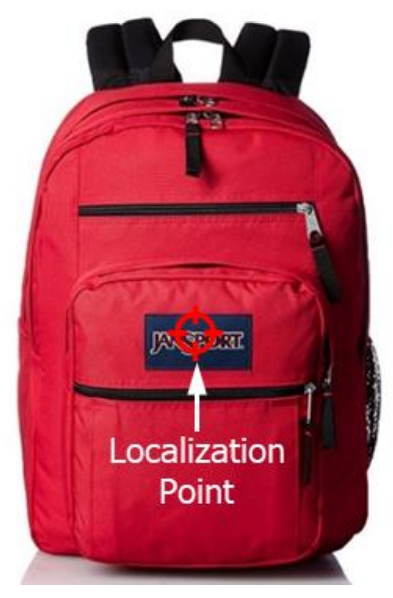
\includegraphics[width=\textwidth]{backpack_artifact.png}
		\caption{Backpack}
		\label{backpack}		
	\end{subfigure}
	\hfill
	\begin{subfigure}{0.32\textwidth}
		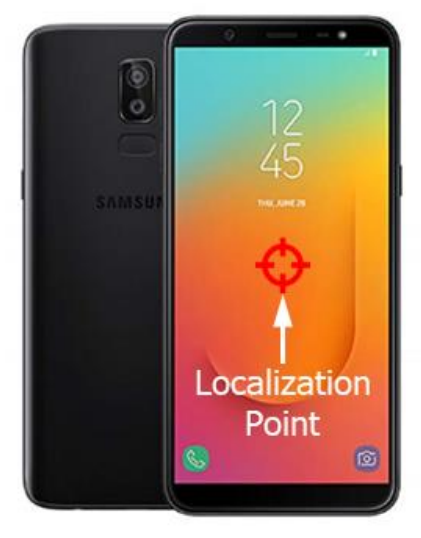
\includegraphics[width=\textwidth]{cell_phone_artifact.png}
		\caption{Cell Phone}
		\label{cell phone}
	\end{subfigure}	
	\hfill
	\begin{subfigure}{0.32\textwidth}
		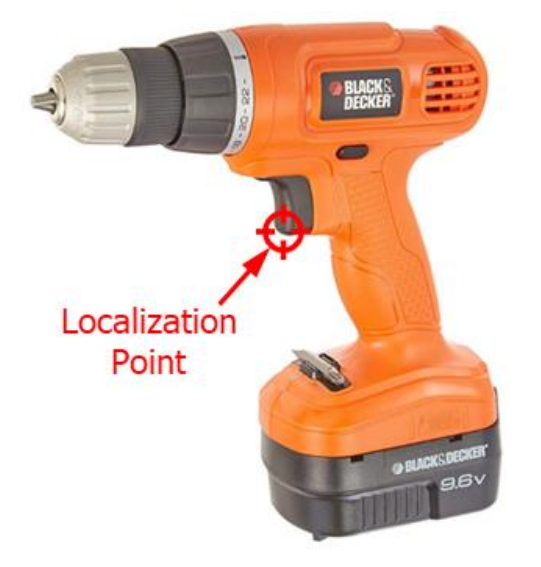
\includegraphics[width=\textwidth]{drill_artifact.png}
		\caption{Drill}
		\label{drill}
	\end{subfigure}
	\\
	\begin{subfigure}{0.47\textwidth}
		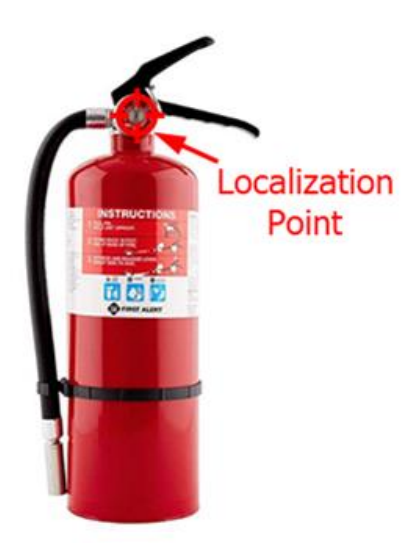
\includegraphics[width=\textwidth]{fire_extinguisher_artifact.png}
		\caption{Fire Extinguisher}
		\label{fire extinguisher}
	\end{subfigure}	
	\hfill
	\begin{subfigure}{0.47\textwidth}
		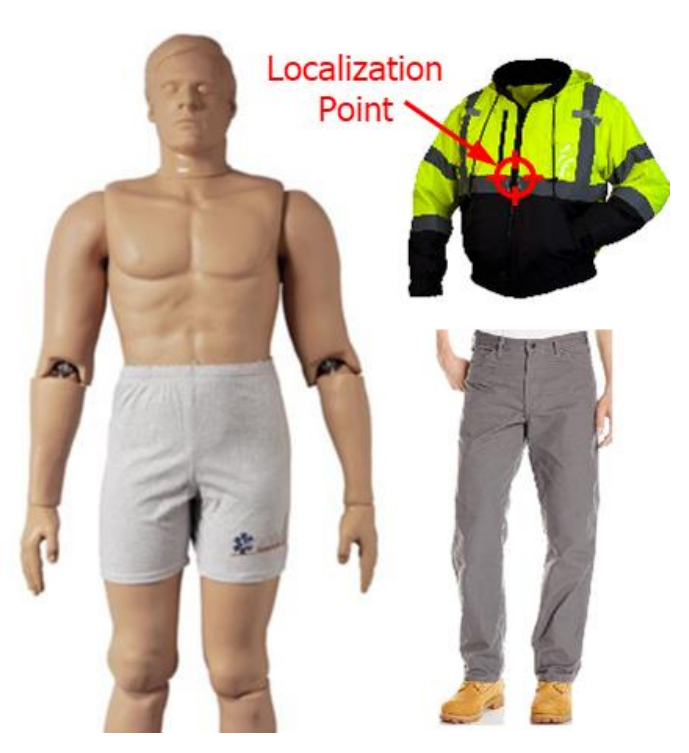
\includegraphics[width=\textwidth]{randy_artifact.png}
		\caption{Survivor ("Randy")}
		\label{randy}
	\end{subfigure}	
	\caption[Tunnel Circuit artifacts]{The Figure depicts the 5 Tunnel Circuit artifacts. The survivor, cell phone, and backpack artifacts are common to all 3 circuit events. Each circuit consists of an additional 2 circuit-specific artifacts, which were the fire extinguisher and drill for the Tunnel Circuit. All 9 artifacts will be used during the final event.}
	\label{tunnel artifacts}
\end{figure}

\section{Related Work}

This work draws inspiration from and extends upon two areas of work -- subterranean mobile robots and multimodal object detection. The early 2000s saw the development of a number of robots intended for use in subterranean environments, such as CMU's Groundhog \cite{ferguson2004autonomous} and CSIRO's Numbat \cite{ralston1998numbat}. These robots were built to specifically address mobility and perception challenges presented by underground mines. They demonstrated considerable mobility in a variety of field experiments, but were limited in their autonomous capabilities by the available compute and sensing technologies \cite{morris2006recent}. Recent advancements in these areas have led to impressive state of the art results in a variety of areas of robot perception, as demonstrated in various tasks on datasets such as ImageNet \cite{deng2009imagenet}, COCO \cite{lin2014microsoft}, and KITTI \cite{Geiger2013IJRR}. Of particular relevance is multimodal object detection, which has seen recent interest due to the necessity for accurate perception by self driving cars in all conditions \cite{feng2019deep}.

\subsection{Subterranean Mobile Robots}

Early subterranean mobile robots like Groundhog were limited in the rapid situational awareness they could provide a basestation operator. Groundhog carried two scanning lasers for mapping and navigation, along with a gyroscope, encoders, and tilt sensors for odometry. 2D maps were generated on board and continually optimized to ensure global consistency, but were not reported to the base station due to a lack of communication infrastructure. The maps could be queried from recorded data after Groundhog returned. Though the fidelity of the maps was high enough to be useful for situational awareness, the high latency of the information could be costly in a disaster response scenario. Even after a base station operator downloaded the maps from the robot, searching the point clouds for specific objects would be a time consuming and inaccurate process done manually.

Other subterranean robots attempted to solve the communication problem with a tether. This enabled robots, such as the MSHA Andros V-2, to report video feeds to the base station in real time. The remote camera acted as a source of more rapid situational awareness than the point clouds from Groundhog, and provided data in a format more easily understandable by humans. However, tethers proved to be unreliable, being prone to tangling and breakage \cite{murphy2009mobile}, and thus unsuitable for disaster response scenarios which require robust solutions. Utilizing such a video streaming system for situational awareness may also prove difficult to scale to multiple robots as human operators would be required to split attention between multiple video feeds and thus potentially miss important moments.

Our work addresses many of the limitations of early systems for providing situational awareness. Each deployed robot in our system autonomously identifies important objects and sends it to the base station over a wireless link. Providing artifacts for situational awareness ensures that the human supervisor receives only high utility information, and reduces the difficulty of operating multiple robots covering a large environment at once. The small size of each artifact also enables transmission over a wireless link even when only low bitrates are available, ensuring real time updates.

\subsection{Multimodal Object Detection}

Multimodal object detection is an important problem for robots as it has the potential to enable more robust perception than any single sensor could. This is especially true for self driving cars, where human lives are at risk. The current best known methods for 2D and 3D object detection, as measured on the KITTI dataset, use deep learning to fuse LIDAR and RGB camera data. \cite{qi2018frustum} performs 2D object detection in RGB images and then projects and refines detections into 3D using LIDAR information. \cite{liang2019multi} instead jointly extracts features from LIDAR and RGB camera data and performs ROI feature fusion.

Unfortunately, these deep fusion methods rely on the availability of large, well labeled datasets to develop high accuracy, and require powerful GPUs to run in real time. Our approach differs by instead using deep learning techniques only to extract 2D bounding boxes from images, which can be done with relatively little training data, and fusing detections with other sensors using classical techniques. Our method for fusing detections from multiple sensing modalities requires only coordinates for each artifact. This allows for the use of additional detection techniques, such as cell phone trilateration \cite{iglesias2012indoor} and sound source localization \cite{grondin2019lightweight}. Work which directly fuses audio and signal strength data in a deep network with LIDAR and RGB data was not found in the literature.